\documentclass{beamer}
\usepackage{amsfonts,amsmath,oldgerm}
\usetheme{sintef}
\usepackage{graphicx}
\usepackage{minted}

\newcommand{\testcolor}[1]{\colorbox{#1}{\textcolor{#1}{test}}~\texttt{#1}}

\usefonttheme[onlymath]{serif}

\titlebackground*{assets/background}

\newcommand{\hrefcol}[2]{\textcolor{cyan}{\href{#1}{#2}}}

\title{Group 10: NXP S32K3X8EVB in QEMU}
\subtitle{Implementation and FreeRTOS porting}
\course{Master's Degree in Computer Science: Embedded Systems}
\author{Francesco Mignone  Leonardo Gallina  Silvia Bonenti  Andrea Baraldi  Lorenzo Parata} 

\begin{document}
\maketitle

\begin{frame}

In this presentation, we will discuss the implementation of the NXP S32K3X8EVB board in QEMU and the porting of FreeRTOS to this architecture.

\vspace{\baselineskip}

This is a collaborative effort by Francesco Mignone, Leonardo Gallina, Silvia Bonenti, Andrea Baraldi, and Lorenzo Parata as part of the Opereting Systems course.

% This template is released under \hrefcol{https://creativecommons.org/licenses/by-nc/4.0/legalcode}{Creative Commons CC BY 4.0} license

\end{frame}

\section{Project Goals}

\begin{frame}{Project Assignment}

    The main goals of this project are:
    \begin{itemize}
        \item {Implement the NXP S32K3X8EVB board in QEMU
            \begin{itemize}
                \item CPU: ARM Cortex-M7
                \item Peripherals: UART, SPI
            \end{itemize}
        }
        \item Port FreeRTOS to the newly implemented architecture
        \item Test the implementation with an application that utilizes the board's peripherals
        \item Document the entire process and provide a comprehensive report
    \end{itemize}
\end{frame}



\section{QEMU Structure}

% \begin{frame}[fragile]{Brief Introduction to QEMU structure}
%     \begin{columns}
%         \begin{column}{0.7\textwidth}
%         Adding images works like in normal \LaTeX:
%         \begin{block}{Code for Adding Images}
%             dsasda
%         \end{block}
%         \end{column}
%         \begin{column}{0.3\textwidth}
%             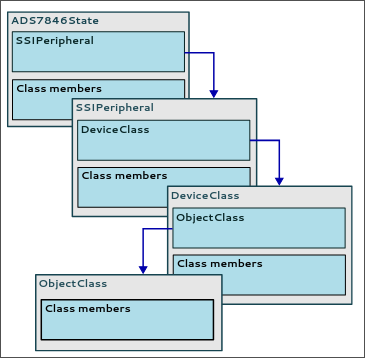
\includegraphics[width=]{assets/qemu_structure.png}
%         \end{column}
%     \end{columns}
% \begin{itemize}
% \end{itemize}
% \end{frame}

\begin{frame}[fragile]{Introduction to QEMU structure}
    \begin{columns}
    \begin{column}{0.6\textwidth}
        Even if QEMU is a complex software, its structure is quite simple and modular:
        \begin{itemize}
            \item Written in C with extra feature that mimics C++ classes
            \item It is composed by a core and several modules organized in parents and children
            \item The core provides the main functionalities, while the modules provide support for different architectures and devices
            \item The main components of QEMU are:
            \begin{itemize}
                \item CPU emulation
                \item Memory management
                \item Device emulation
                \item I/O handling
            \end{itemize}
        \end{itemize}
    \end{column}
    \begin{column}{0.4\textwidth}
            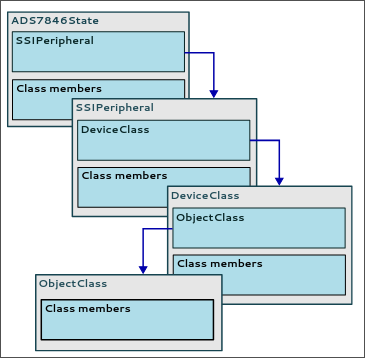
\includegraphics[width=\textwidth]{assets/qemu_structure.png}
    \end{column}
    \end{columns}
\end{frame}

\begin{frame}[fragile]{Basic QEMU Module}
    Each module in QEMU has two main phases:
    \begin{itemize}
        \item Initialization: where the module is registered and its properties are set
        \item Realization: where the module interacts with other components and performs its functions
    \end{itemize}
\end{frame}

\section{QEMU Implementation}

\footlinecolor{}
\begin{frame}[fragile]{NXP S32K3X8EVB}
    The Board has been divided in two components for modularity:
    \begin{itemize}
        \item MCU: with CPU and peripherals (UART, SPI)
        \item Main Board: mounts the MCU and can be used to attach other components in the future
    \end{itemize}
\end{frame}

\begin{frame}[fragile]{Board Declaration}
    \begin{columns}
        \begin{column}{0.5\textwidth}
            The MCU includes:
            \begin{itemize}
                \item ARM Cortex-M7 CPU
                \item 512KB SRAM
                \item 1MB Flash memory
                \item UART peripherals
                \item SPI peripherals
            \end{itemize}
        \end{column}
        \begin{column}{0.5\textwidth}
            \begin{block}{MCU Initialization}
                    \begin{footnotesize}
                        \begin{verbatim}
struct S32K3x8State{
    SysBusDevice parent_obj;
    ARMv7MState cpu;
    Clock *sysclk;
    uint32_t sram0_size;    
    uint32_t flash0_size;  
    MemoryRegion sram0;
    MemoryRegion flash0;
    MemoryRegion flash_alias;
    MemoryRegion *board_memory;
    MemoryRegion container;
    S32K3x8UartState uart[NXP_NUM_UARTS];
    S32K3x8SPIState spi[NXP_NUM_SPI];
};
                        \end{verbatim}
                    \end{footnotesize}
            \end{block}
        \end{column}
    \end{columns}
\end{frame}

\footlinecolor{}
\begin{frame}[fragile]{UART}

\begin{columns}
    \begin{column}{0.5\textwidth}
        The UART peripheral has been implemented with the following features:
        \begin{itemize}
            \item Basic configuration (baud rate, data bits, stop bits, parity)
            \item Data transmission and reception
            \item Interrupt handling
        \end{itemize}
        All 16 UARTs have been implemented, but only UART0 has been tested, since the code is the same, with base address \mintinline{c}|0x40328000|    
    \end{column}
    \begin{column}{0.5\textwidth}
        \begin{block}{MCU Initialization}
                \begin{footnotesize}
                    \begin{verbatim}
struct S32K3x8UartState {
    SysBusDevice parent_obj;
    MemoryRegion mmio;
    uint32_t usart_sr;
    uint32_t usart_dr;
    uint32_t usart_brr;
    uint32_t usart_cr1;
    uint32_t usart_cr2;
    uint32_t usart_cr3;
    uint32_t usart_gtpr;
    CharBackend chr;
    qemu_irq irq;
};
                    \end{verbatim}
                \end{footnotesize}
        \end{block}
    \end{column}
\end{columns}
\end{frame}

\footlinecolor{}
\begin{frame}[fragile]{SPI}
    \begin{columns}
        \begin{column}{0.5\textwidth}
            The SPI peripheral implementation includes:
            \begin{itemize}
                \item Basic configuration and initialization
                \item Data transmission and reception
                \item Interrupt handling
            \end{itemize}
            Since there is no effective device at the end of the SPI bus, the implementation is done by saving the written data and returning incremented by one on read.
        \end{column}
        \begin{column}{0.5\textwidth}
            \begin{block}{MCU Initialization}
                    \begin{footnotesize}
                        \begin{verbatim}
struct S32K3x8SPIState {
    SysBusDevice parent_obj;
    MemoryRegion mmio;
    uint32_t spi_cr1;
    uint32_t spi_cr2;
    uint32_t spi_sr;
    uint32_t spi_dr;
    uint32_t spi_crcpr;
    uint32_t spi_rxcrcr;
    uint32_t spi_txcrcr;
    uint32_t spi_i2scfgr;
    uint32_t spi_i2spr;
    uint32_t test_var;
    qemu_irq irq;
    SSIBus *ssi;
};
                        \end{verbatim}
                    \end{footnotesize}
            \end{block}
        \end{column}
    \end{columns}
\end{frame}



\section{FreeRTOS Porting}

\footlinecolor{}
\begin{frame}[fragile]{FreeRTOS Porting}
    The porting of FreeRTOS to the NXP S32K3X8EVB architecture involved several steps:
    \begin{itemize}
        \item Setting up the development environment
        \item Configuring FreeRTOS for the ARM Cortex-M7 architecture
        \item Testing and debugging the ported FreeRTOS on the QEMU-emulated board
    \end{itemize}
\end{frame}

\footlinecolor{}
\begin{frame}[fragile]{Development Environment}
    The development environment was set up with the following tools:
    \begin{itemize}
        \item GCC toolchain for ARM
        \item FreeRTOS source code
        \item Makefile for building and linking the application
    \end{itemize}
\end{frame}

\footlinecolor{}
\begin{frame}[fragile]{Peripheral test: UART}
    \begin{columns}
        \begin{column}{0.5\textwidth}
            The test application for the UART peripheral includes:
            \begin{itemize}
                \item Initialization of the UART peripheral
                \item Sending data
                \item Printing messages to the terminal
            \end{itemize}
            The application is structured as a FreeRTOS task that runs independently.
        \end{column}
        \begin{column}{0.5\textwidth}
            \begin{block}{MCU Initialization}
                    \begin{footnotesize}
                        \begin{verbatim}
int main(int argc, char **argv) {
...
    UART_init();
...
}
...
void UART_test(void *pvParameters) {
(void)pvParameters;
uart_printf("Starting UART Test\n");
uart_printf("Hello from UART of Group10!\n");
uart_printf("Ending UART Test\n");
vTaskDelete(NULL);
}
                        \end{verbatim}
                    \end{footnotesize}
            \end{block}
        \end{column}
    \end{columns}
\end{frame}

\footlinecolor{}
\begin{frame}[fragile]{Peripheral test: SPI}
    \begin{columns}
        \begin{column}{0.5\textwidth}
            The test application for the SPI peripheral includes:
            \begin{itemize}
                \item Initialization of the SPI peripheral
                \item Sending and receiving data
                \item Printing messages to the terminal
            \end{itemize}
            Also this application is structured as a FreeRTOS task that runs independently.
        \end{column}
        \begin{column}{0.5\textwidth}
            \begin{block}{MCU Initialization}
                    \begin{footnotesize}
                        \begin{verbatim}
int main(int argc, char **argv) {
    SPI_init();
}
void SPI_test(void *pvParameters) {
  (void)pvParameters;
  SPI_status();
  uint32_t pippo = 0x00;
  uint32_t pluto = 0x00;
  for (int i=0; i<10; ++i) {
    uart_printf("Sending: %x\n", pippo);
    SPI_write((uint8_t)pippo);
    SPI_get((uint8_t *)&pluto);
    pippo = pluto;
    uart_printf("SPI read: %x\n", pluto);
    vTaskDelay(pdMS_TO_TICKS(1000));
  }
  SPI_status();
  }
                        \end{verbatim}
                    \end{footnotesize}
            \end{block}
        \end{column}
    \end{columns}
\end{frame}


\begin{frame}
\frametitle{Teast Output}
    \begin{center}
        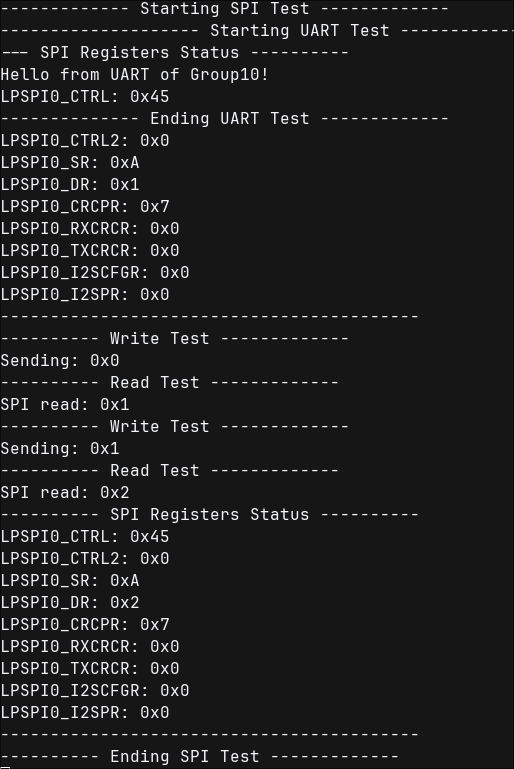
\includegraphics[height=\textheight]{assets/test_output.png}
    \end{center}
\end{frame}

\section{Summary}

\begin{frame}
\frametitle{Conclusions}
    In conclusion, the implementation of the NXP S32K3X8EVB board in QEMU and the porting of FreeRTOS to this architecture were successful. The main achievements include:
    \begin{itemize}
        \item Successful implementation of the NXP S32K3X8EVB board in QEMU, including CPU and peripherals (UART, SPI)
        \item Porting of FreeRTOS to the ARM Cortex-M7 architecture
        \item Development and testing of applications that utilize the board's peripherals
        \item Comprehensive documentation of the entire process
    \end{itemize}
    
    Future work could involve adding more peripherals, improving the existing implementations, and exploring additional features of FreeRTOS.
\end{frame}

\backmatter
\end{document}
